\documentclass[11pt]{article}
\usepackage[spanish]{babel}
\usepackage[utf8]{inputenc}
\usepackage{amsmath}
\usepackage{geometry}
\usepackage{graphicx}
\usepackage{listings}
\usepackage{xcolor}
\usepackage{float}
\graphicspath{{images/}}
\geometry{margin=2.5cm}

\definecolor{matlabkeyword}{rgb}{0,0,1}
\definecolor{matlabcomment}{rgb}{0.13,0.55,0.13}
\definecolor{matlabstring}{rgb}{0.63,0.13,0.94}
\definecolor{matlabbg}{rgb}{0.97,0.97,0.97}

\lstdefinelanguage{Matlab}{
  keywords={break,case,catch,continue,else,elseif,end,for,function,global,if,otherwise,persistent,return,switch,try,while},
  keywordstyle=\color{matlabkeyword}\bfseries,
  sensitive=true,
  comment=[l]{\%},
  commentstyle=\color{matlabcomment}\itshape,
  string=[b]',
  stringstyle=\color{matlabstring},
  morestring=[b]"
}

\lstset{
  language=Matlab,
  backgroundcolor=\color{matlabbg},
  basicstyle=\ttfamily\small,
  breaklines=true,
  columns=fullflexible,
  frame=single,
  numbers=left,
  numberstyle=\tiny\color{gray},
  showstringspaces=false
}

\title{Taller Potencia}
\author{}
\date{}

\begin{document}
\maketitle

Valores de los elementos: $a=9$, $b=2$, $c=6$

\setcounter{section}{1}

\section{Rectificador Trif\'asico de Media Onda}

\subsection{Enunciado}

El rectificador trif\'asico de media onda de la figura se alimenta con
$V_f = 352.76\,V\,\sin(100\pi t)$; $R = 88\,\Omega$; $L = 10\,mH$. Se pide
definir la se\~nal de salida entre $-T_0/2$ y $T_0/2$ para obtener los
t\'erminos de la serie de Fourier. Calcule: $a_0$, $a_1$, $b_1$, $a_n$ y $b_n$
mediante integraci\'on de las funciones de la serie. Dibuje las se\~nales de
$v_o$ e $i_o$ resultantes (anexando c\'odigo y gr\'aficas). Calcule las
tensiones y corrientes eficaces, las potencias $P$, $P_{DC}$, $I_{DC}$, $I_L$,
$S$, el factor de potencia ($fp$), la eficiencia ($\eta$) y los factores de
rizado ($FR$). Realice la simulaci\'on, verifique los resultados, calcule los
par\'ametros no medidos y determine los errores de todos los valores te\'oricos
respecto a los simulados.

\begin{figure}[H]
\centering
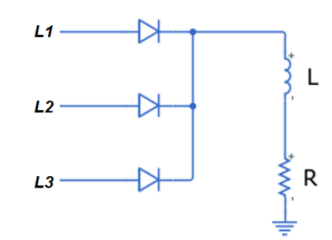
\includegraphics[width=0.45\textwidth]{ej2_rectificador_trifasico_media_onda_circuito_figura9.png}
\caption{Rectificador Trif\'asico de Media Onda}
\end{figure}

\subsection{Soluci\'on Anal\'itica}

Para los par\'ametros del circuito (f\'ormulas dadas en el enunciado del taller:
$R = 8(a+b)\,\Omega$ y $L = (2b+c)\,mH$):

\begin{align*}
R &= 8(a+b)\,\Omega = 8(9+2)\,\Omega = \boxed{88\,\Omega} \\
L &= (2b+c)\,mH = (2(2)+6)\,mH = \boxed{10\,mH} = \boxed{0.01\,H} \\
V_f &= \frac{V_L}{\sqrt{3}} = \boxed{352.76\,V}, \qquad f = \boxed{50\,Hz}
\end{align*}

Para un rectificador trif\'asico de media onda, el periodo fundamental de la
se\~nal de salida es una tercera parte del per\'iodo de entrada. F\'ormula
general: $T_0 = \dfrac{T}{p} = \dfrac{1}{p\,f}$, con $p=3$ pulsos.

\begin{align*}
T_0 = \frac{1}{3f} = \frac{1}{150\,Hz} = \boxed{6.67\,ms}
\end{align*}

\textbf{Componente DC} ($n=0$, $f=0\,Hz$). Como la se\~nal de salida se repite
cada $2\pi/3$ y cada fase conduce entre $\pi/6$ y $5\pi/6$, la f\'ormula
general es:
$V_{DC} = \dfrac{1}{2\pi/3}\displaystyle\int_{\pi/6}^{5\pi/6} V_m\,\sin\theta\,d\theta
= \dfrac{3V_m}{2\pi}\left[-\cos\theta\right]_{\pi/6}^{5\pi/6}$.

\begin{align*}
V_0 = V_{DC} &= \frac{1}{\frac{2\pi}{3}}\int_{\pi/6}^{5\pi/6} 352.76\,\sin(\theta)\,d\theta
= \frac{3(352.76)}{2\pi}\left[-\cos\!\left(\frac{5\pi}{6}\right)-\left(-\cos\!\left(\frac{\pi}{6}\right)\right)\right]
= \boxed{291.73\,V}
\end{align*}

F\'ormula general de la corriente DC (la bobina no cae tensi\'on en DC):
$I_{DC} = V_{DC}/R$.

\begin{align*}
I_{DC} = \frac{291.73\,V}{88\,\Omega} = \boxed{3.32\,A}
\end{align*}

\subsection{Definici\'on de la se\~nal en $\left[-\frac{T_0}{2},\frac{T_0}{2}\right]$ y Serie de Fourier}

Para obtener los t\'erminos de la serie de Fourier mediante integraci\'on,
definimos la se\~nal de salida centrada en el intervalo sim\'etrico
$\left[-\frac{T_0}{2},\frac{T_0}{2}\right]$ (que en el dominio angular
corresponde a $\left[-\frac{\pi}{3},\frac{\pi}{3}\right]$):

Al centrar el intervalo, el pico de la fase que conduce queda en $\theta=0$
(la fase conduce de $-\pi/3$ a $\pi/3$ alrededor de su m\'aximo), por lo que la
se\~nal es una funci\'on coseno:

\begin{align*}
v_o(\theta) = 352.76\,\cos(\theta) \quad \text{para} \quad -\frac{\pi}{3}\le\theta\le\frac{\pi}{3}
\end{align*}

La se\~nal es par y de periodo $\Theta = 2\pi/3$, as\'i que solo aparecen
arm\'onicos m\'ultiplos de 3 ($n=3,6,9,\dots$) y todos los $b_n$ valen $0$.

Los coeficientes de la serie de Fourier se calculan mediante integraci\'on en
dicho intervalo. F\'ormulas generales, con $\Theta = 2\pi/3$:
$a_0 = \dfrac{1}{\Theta}\displaystyle\int v_o\,d\theta$, \quad
$a_n = \dfrac{2}{\Theta}\displaystyle\int v_o\cos(n\theta)\,d\theta$, \quad
$b_n = \dfrac{2}{\Theta}\displaystyle\int v_o\sin(n\theta)\,d\theta$.

\textbf{C\'alculo de $a_0$}

\begin{align*}
a_0 = \frac{1}{\frac{2\pi}{3}}\int_{-\pi/3}^{\pi/3} 352.76\,\cos(\theta)\,d\theta
= \frac{3(352.76)}{2\pi}\left[\sin(\theta)\right]_{-\pi/3}^{\pi/3}
= \frac{3(352.76)}{2\pi}\left[\sin\!\left(\frac{\pi}{3}\right)-\sin\!\left(-\frac{\pi}{3}\right)\right]
= \boxed{291.73\,V}
\end{align*}

\textbf{C\'alculo de $a_1$ y $b_1$ (Primer arm\'onico)}

La salida se repite cada $2\pi/3$, por lo que no contiene la componente de la
frecuencia de entrada ($n=1$, $50\,Hz$); el primer arm\'onico presente es $n=3$.
Por lo tanto:

\begin{align*}
a_1 = \boxed{0\,V}, \qquad b_1 = \boxed{0\,V}
\end{align*}

\textbf{C\'alculo de $a_n$ y $b_n$ (Arm\'onicos generales y orden $n=3$)}

Para un arm\'onico de orden $n$ gen\'erico ($n$ m\'ultiplo de 3):

\begin{align*}
a_n &= \frac{3}{\pi}\int_{-\pi/3}^{\pi/3} 352.76\,\cos(\theta)\cos(n\theta)\,d\theta \\
b_n &= \frac{3}{\pi}\int_{-\pi/3}^{\pi/3} 352.76\,\cos(\theta)\sin(n\theta)\,d\theta = 0\,V
\end{align*}

($b_n = 0$ porque el integrando $\cos(\theta)\sin(n\theta)$ es impar en un
intervalo sim\'etrico.)

Para el tercer arm\'onico significativo ($n=3$, $f=150\,Hz$):

\begin{align*}
a_3 &= \frac{3}{\pi}\int_{-\pi/3}^{\pi/3} 352.76\,\cos(\theta)\cos(3\theta)\,d\theta = \boxed{72.93\,V} \\
b_3 &= \frac{3}{\pi}\int_{-\pi/3}^{\pi/3} 352.76\,\cos(\theta)\sin(3\theta)\,d\theta = \boxed{0\,V}
\quad \text{(componente principal de rizado)}
\end{align*}

Magnitud de la componente de 150\,Hz. F\'ormula general: $V_n = \sqrt{a_n^2 + b_n^2}$.

\begin{align*}
V_3 = \sqrt{(72.93\,V)^2 + (0\,V)^2} = \boxed{72.93\,V}
\end{align*}

Impedancia vista por el tercer arm\'onico ($\omega_3 = 300\pi\ rad/s$). F\'ormula
general: $Z_n = R + j\,n\omega L$, con $n\omega = 3(100\pi) = 300\pi$.

\begin{align*}
Z_3 = 88\,\Omega + j\left(300\pi\,\tfrac{rad}{s}\right)(0.01\,H) = 88 + j9.42 = \boxed{88.50\,\Omega\angle 0.11\,r}
\end{align*}

Corriente del tercer arm\'onico. F\'ormula general: $I_n = \dfrac{V_n\angle 0}{Z_n}$.

\begin{align*}
I_3 = \frac{72.93\,V\angle 0\,r}{88.50\,\Omega\angle 0.11\,r} = \boxed{0.82\,A\angle -0.11\,r}
\end{align*}

\subsection{Valores promedio y eficaces de tensiones y corrientes}

Corriente eficaz de salida. F\'ormula general (los arm\'onicos entran con su valor
pico, por eso se divide entre 2 dentro de la ra\'iz):
$I_{rms} = \sqrt{I_{DC}^2 + \dfrac{I_3^2}{2}}$.

\begin{align*}
I_{rms} = \sqrt{(3.32\,A)^2 + \frac{(0.82\,A)^2}{2}} = \boxed{3.37\,A}
\end{align*}

Tensi\'on eficaz de salida. F\'ormula general:
$V_{rms} = \sqrt{V_{DC}^2 + \dfrac{V_3^2}{2}}$.

\begin{align*}
V_{rms} = \sqrt{(291.73\,V)^2 + \frac{(72.93\,V)^2}{2}} = \boxed{296.25\,V}
\end{align*}

Corriente eficaz de l\'inea (cada fase conduce un tercio del ciclo). F\'ormula
general: $I_L = I_{rms}/\sqrt{3}$.

\begin{align*}
I_L = \frac{I_{rms}}{\sqrt{3}} = \frac{3.37\,A}{\sqrt{3}} = \boxed{1.95\,A}
\end{align*}

\subsection{Potencias activa, aparente y DC}

Usando el valor RMS del voltaje de fase de entrada
($V_{f,rms} = \frac{352.76}{\sqrt{2}} = 249.44\,V$). F\'ormulas generales:
$S = 3\,V_{f,rms}\,I_L$, \quad $P = I_{rms}^2\,R$, \quad $P_{DC} = V_{DC}\,I_{DC}$.

\begin{align*}
S &= 3(249.44\,V)(1.95\,A) = \boxed{1459.2\,VA} \\
P &= (3.37\,A)^2(88\,\Omega) = \boxed{999.4\,W} \\
P_{DC} &= (291.73\,V)(3.32\,A) = \boxed{968.5\,W}
\end{align*}

\subsection{Par\'ametros de rendimiento}

Factor de potencia. F\'ormula general: $f_p = P/S$.

\begin{align*}
f_p = \frac{999.4\,W}{1459.2\,VA} = \boxed{0.685}
\end{align*}

Eficiencia (en este ejercicio se define respecto a $P$). F\'ormula general:
$\eta = P_{DC}/P$.

\begin{align*}
\eta = \frac{968.5\,W}{999.4\,W} = \boxed{0.969}\ (96.9\,\%)
\end{align*}

Factor de rizado en tensi\'on. F\'ormula general: $FR_V = \dfrac{V_3/\sqrt{2}}{V_{DC}}$.

\begin{align*}
FR_V = \frac{72.93\,V/\sqrt{2}}{291.73\,V} = \boxed{0.177}
\end{align*}

Factor de rizado en corriente. F\'ormula general: $FR_I = \dfrac{I_3/\sqrt{2}}{I_{DC}}$.

\begin{align*}
FR_I = \frac{0.82\,A/\sqrt{2}}{3.32\,A} = \boxed{0.175}
\end{align*}

\subsection{Especificaciones del puente rectificador}

Corriente eficaz por diodo (conducci\'on $1/3$ del ciclo). F\'ormula general:
$I_{D,rms} = I_{rms}/\sqrt{3}$.

\begin{align*}
I_{D,rms} = \frac{I_{rms}}{\sqrt{3}} = \frac{3.37\,A}{\sqrt{3}} = \boxed{1.95\,A}
\end{align*}

\subsection{Dibujo de se\~nales}

\subsubsection{Definiciones}

La se\~nal del voltaje de salida est\'a dada por:
\begin{align*}
v_o(t) = 291.73\,V + 72.93\,V\cos(300\pi t) + \dots
\end{align*}

Mientras que la funci\'on de corriente definida en el tiempo es:
\begin{align*}
i_o(t) = 3.32\,A + 0.82\,A\cos(300\pi t - 0.11\,r) + \dots
\end{align*}

\subsubsection{C\'odigo}

Los c\'odigos en MATLAB para realizar las gr\'aficas de las se\~nales son:

\begin{lstlisting}[language=Matlab, caption={Voltaje de salida}, label={lst:ej2vo}]
t = linspace(0, 20e-3, 300); vo = 291.73 + 72.93*cos(300*pi*t);
plot(t, vo, 'b', 'LineWidth', 1.5); grid on
title('Tension de salida Vo'); xlabel('Tiempo (s)'); ylabel('Voltaje (V)');
\end{lstlisting}

\begin{lstlisting}[language=Matlab, caption={Corriente de salida}, label={lst:ej2io}]
t = linspace(0, 20e-3, 300); io = 3.32 + 0.82*cos(300*pi*t - 0.11);
plot(t, io, 'r', 'LineWidth', 1.5); grid on
title('Corriente de salida Io'); xlabel('Tiempo (s)'); ylabel('Corriente (A)');
\end{lstlisting}

\subsubsection{Gr\'aficas resultantes}

La Figura~\ref{fig:vomatlab2} muestra la tensi\'on de salida $V_o$ en funci\'on
del tiempo, obtenida mediante simulaci\'on en MATLAB para un periodo de red
(20 ms). La se\~nal oscila alrededor de un valor medio de 291.73 V, presentando
3 pulsos completos correspondientes a la componente arm\'onica de tercer orden
(150 Hz).

\begin{figure}[H]
\centering
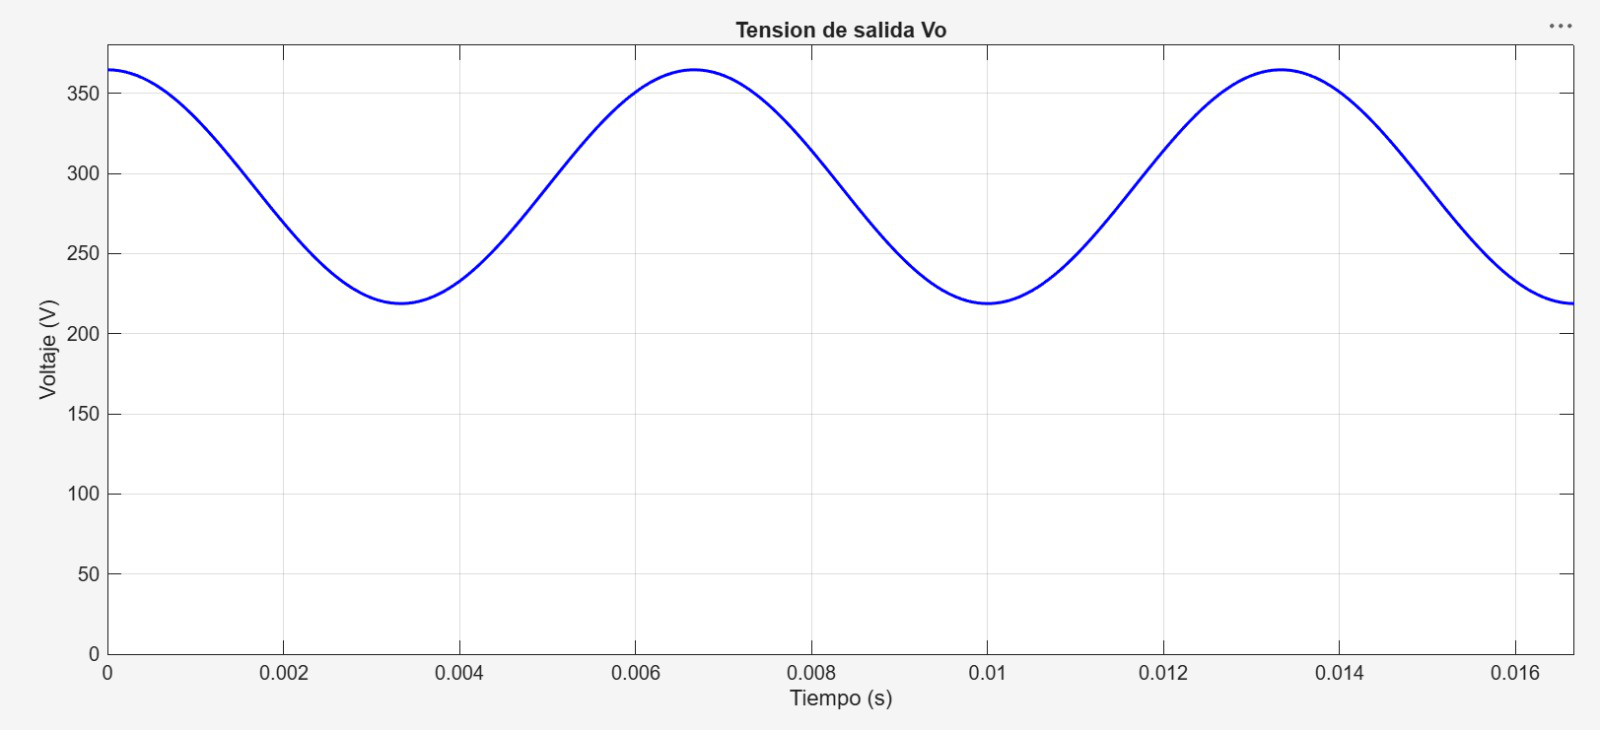
\includegraphics[width=0.9\textwidth]{ej2_tension_salida_vo_grafica_matlab_periodo_20ms.png}
\caption{Tensi\'on de salida Vo}
\label{fig:vomatlab2}
\end{figure}

\begin{figure}[H]
\centering
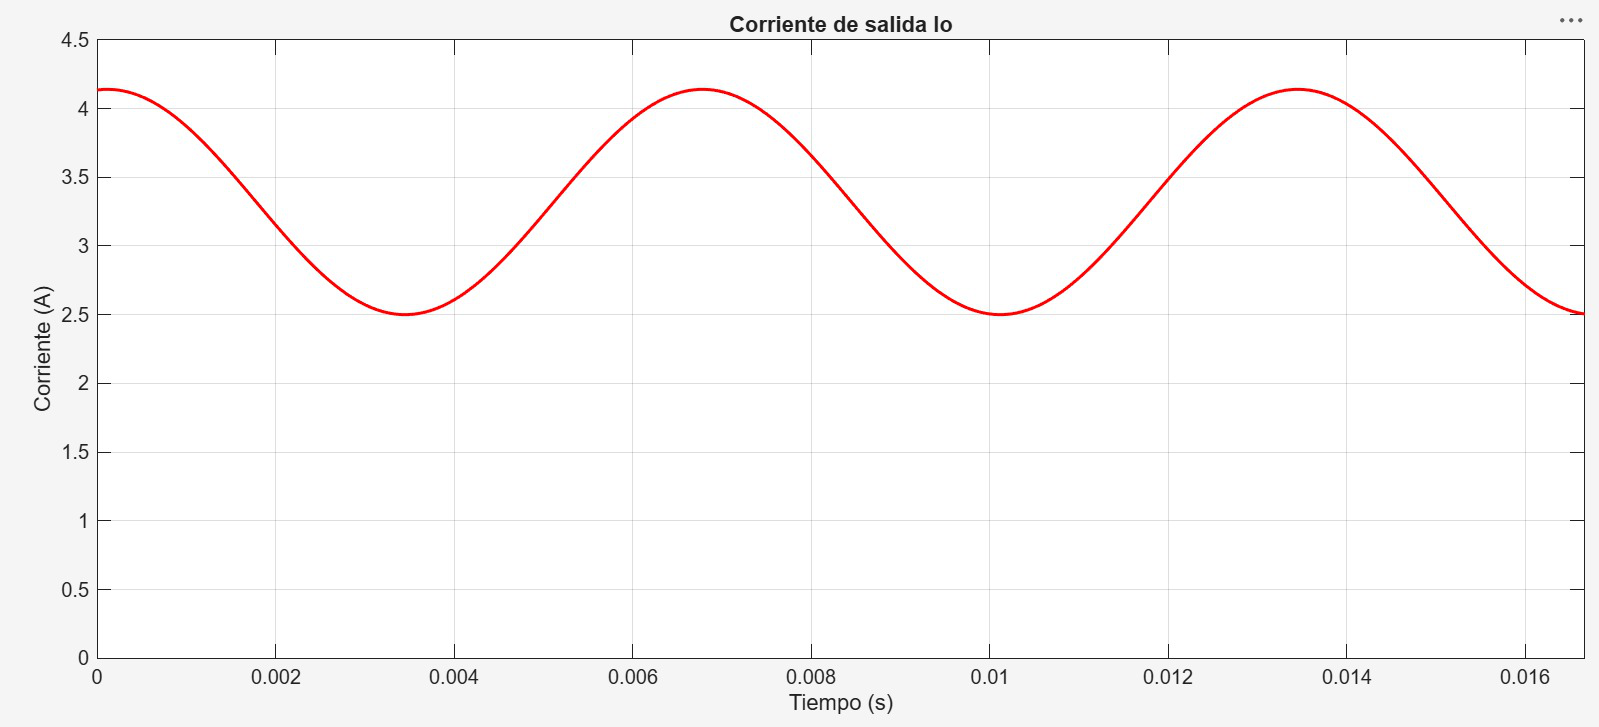
\includegraphics[width=0.9\textwidth]{ej2_corriente_salida_io_grafica_matlab_periodo_20ms.png}
\caption{Corriente de salida Io}
\end{figure}

\subsection{Simulaciones}

La simulaci\'on se realiz\'o en Simscape de MATLAB. Las se\~nales obtenidas en
esta simulaci\'on se muestran a continuaci\'on.

\subsubsection{Mediciones de tensiones y corrientes}

\begin{figure}[H]
\centering
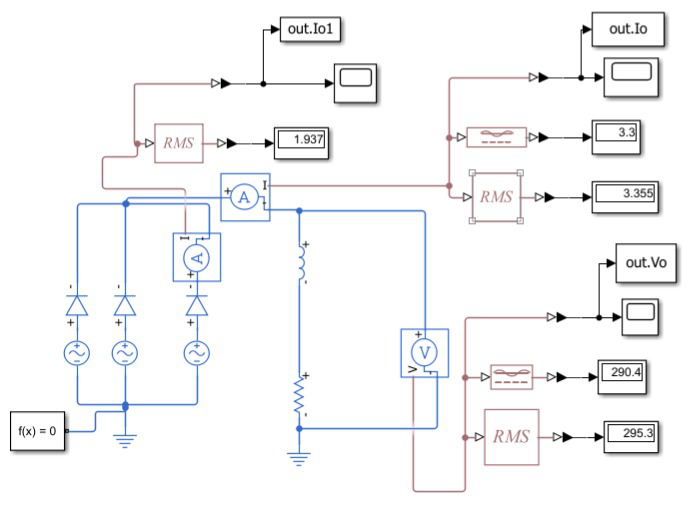
\includegraphics[width=0.75\textwidth]{ej2_simulacion_simscape_mediciones_trifasico_media_onda.png}
\caption{Simulaci\'on del Rectificador Trif\'asico de Media Onda}
\label{fig:sim2}
\end{figure}

\subsubsection{Se\~nales de simulaci\'on}

\begin{figure}[H]
\centering
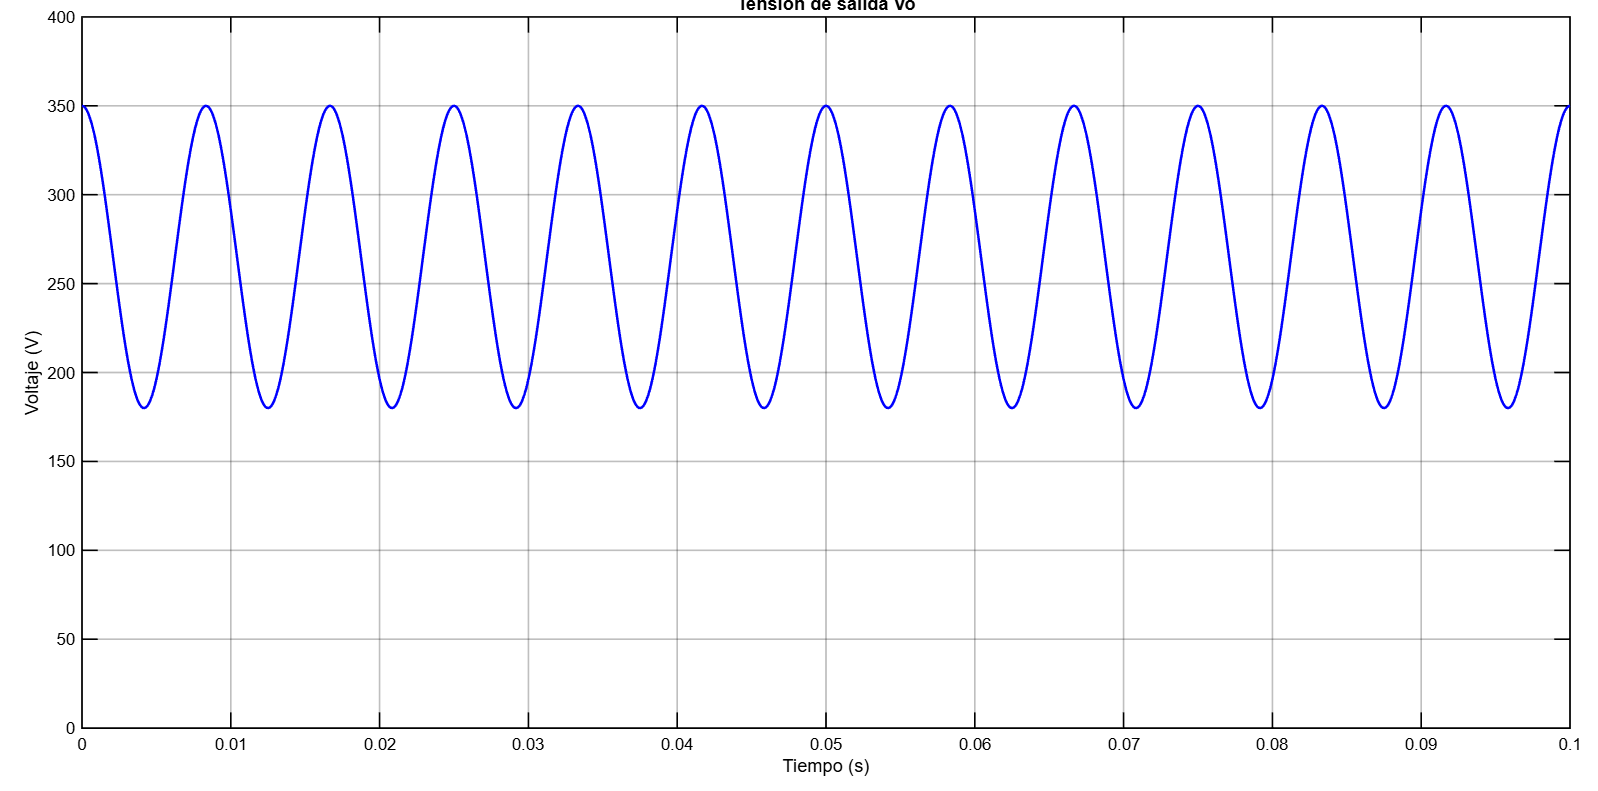
\includegraphics[width=0.95\textwidth]{ej2_simulacion_senal_voltaje_salida_vo.png}
\caption{Se\~nal de voltaje de salida v(t)}
\end{figure}

\begin{figure}[H]
\centering
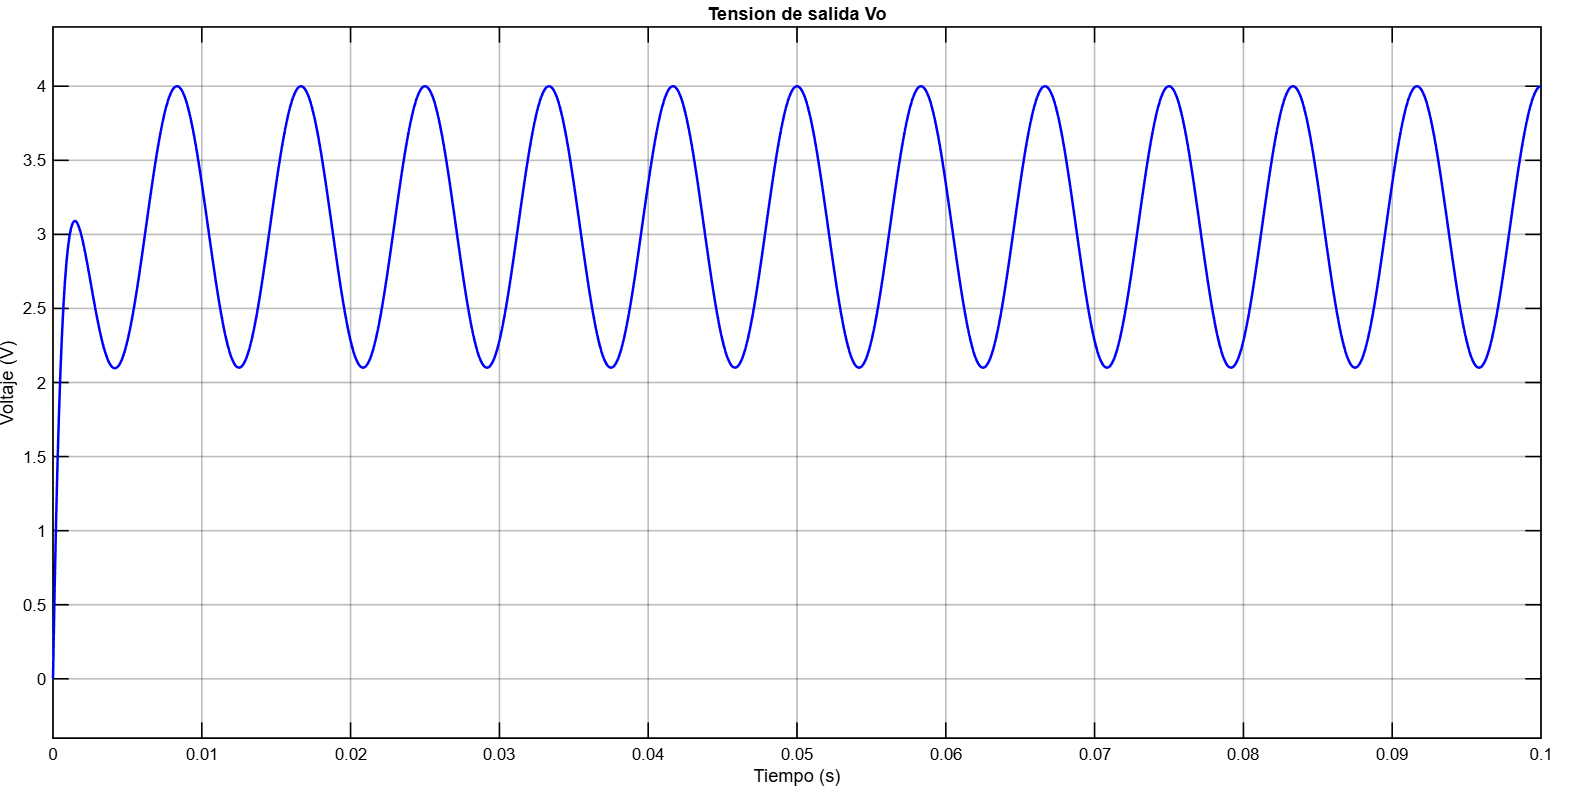
\includegraphics[width=0.95\textwidth]{ej2_simulacion_senal_corriente_salida_io.png}
\caption{Se\~nal de corriente de salida}
\end{figure}

\subsection{C\'alculos con los datos de simulaci\'on}

En la nueva simulaci\'on se obtuvieron los siguientes resultados de las
pantallas (Displays) (ver Figura~\ref{fig:sim2}):

\begin{align*}
V_{DC} = 290.4\,V, \qquad V_{RMS} = 295.3\,V, \qquad I_{DC} = 3.30\,A \\
I_{RMS} = 3.355\,A, \qquad I_L = 1.937\,A, \qquad I_{D,rms} = 1.937\,A
\end{align*}

Con estos datos se procede a realizar los c\'alculos de los dem\'as par\'ametros
(con las mismas f\'ormulas generales de las secciones 2.5 y 2.6).

La potencia activa en la carga es ($P = I_{RMS}^2\,R$):
\begin{align*}
P = (3.355\,A)^2(88\,\Omega) = \boxed{991\,W}
\end{align*}

La potencia aparente en la fuente, utilizando $V_{f,rms} = 249.44\,V$, es
($S = 3\,V_{f,rms}\,I_L$):
\begin{align*}
S = 3(249.44\,V)(1.937\,A) = \boxed{1.45\times10^{3}\,VA}
\end{align*}

La potencia DC obtenida es ($P_{DC} = V_{DC}\,I_{DC}$):
\begin{align*}
P_{DC} = (290.4\,V)(3.30\,A) = \boxed{958\,W}
\end{align*}

El factor de potencia es ($f_p = P/S$):
\begin{align*}
f_p = \frac{991\,W}{1.45\times10^{3}\,VA} = \boxed{0.683}
\end{align*}

La eficiencia es ($\eta = P_{DC}/P$):
\begin{align*}
\eta = \frac{958\,W}{991\,W} = \boxed{0.967}
\end{align*}

Factores de rizado a partir de los valores RMS y DC. F\'ormula general:
$FR = \dfrac{\sqrt{RMS^2 - DC^2}}{DC}$.

Para la tensi\'on:
\begin{align*}
FR_V = \frac{\sqrt{(295.3\,V)^2 - (290.4\,V)^2}}{290.4\,V} = \boxed{0.184}
\end{align*}

Para la corriente:
\begin{align*}
FR_I = \frac{\sqrt{(3.355\,A)^2 - (3.30\,A)^2}}{3.30\,A} = \boxed{0.183}
\end{align*}

\subsection{Comparaci\'on de resultados}

F\'ormula general del error (tomando los valores calculados como referencia):
$Error\,\% = \dfrac{|Valor_{calculado} - Valor_{simulaci\acute{o}n}|}{Valor_{calculado}}\times 100$.

\begin{center}
\textbf{Tabla 2:} Comparaci\'on de Par\'ametros Calculados y Simulados

\medskip
\begin{tabular}{|l|c|c|c|}
\hline
\textbf{\textcolor{blue}{Par\'ametros}} & \textbf{\textcolor{blue}{Valor Calculado}} & \textbf{\textcolor{blue}{Valor de Simulaci\'on}} & \textbf{\textcolor{red}{Error \%}} \\ \hline
$V_{DC}$ (V) & 291.73 & 290.4 & 0.456 \\
$V_{RMS}$ (V) & 296.25 & 295.3 & 0.321 \\
$I_{DC}$ (A) & 3.32 & 3.30 & 0.602 \\
$I_{RMS}$ (A) & 3.37 & 3.355 & 0.445 \\
$I_L$ (A) & 1.95 & 1.937 & 0.667 \\
$I_{D,rms}$ (A) & 1.95 & 1.937 & 0.667 \\
$P$ (W) & 999.4 & 991 & 0.888 \\
$S$ (VA) & 1459.2 & 1449 & 0.665 \\
$P_{DC}$ (W) & 968.5 & 958 & 1.05 \\
$f_p$ & 0.685 & 0.683 & 0.239 \\
$\eta$ & 0.969 & 0.967 & 0.157 \\
$FR_V$ & 0.177 & 0.184 & 4.22 \\
$FR_I$ & 0.175 & 0.183 & 4.76 \\ \hline
\end{tabular}
\end{center}

\end{document}
